% !TeX program = pdflatex

%========================
% Econ_Conj.tex
%========================
\documentclass[11pt]{article}

%---- Page & fonts
\usepackage[margin=1in]{geometry}
\usepackage[T1]{fontenc}
\usepackage[utf8]{inputenc}
\DeclareUnicodeCharacter{2013}{--}   % en dash
\DeclareUnicodeCharacter{2014}{---}  % em dash
\DeclareUnicodeCharacter{2212}{-}    % unicode minus
\DeclareUnicodeCharacter{00D7}{\times}
\usepackage{lmodern}
\usepackage[american]{babel}
\usepackage{microtype}
\usepackage{authblk}
\usepackage{setspace}

%---- Math & symbols
\usepackage{amsmath, amssymb, mathtools}
\usepackage{bbm}
\usepackage{siunitx}
\usepackage{csquotes}

%---- Graphics, tables, floats
\usepackage{graphicx}
\usepackage{xcolor}
\usepackage{booktabs, threeparttable, tabularx}
\usepackage{caption}
\usepackage{subcaption}
\usepackage{float}
\usepackage{placeins}
\usepackage{tikz}
\usetikzlibrary{decorations.pathreplacing}
\definecolor{ecblue}{HTML}{184E77}
\definecolor{eclight}{HTML}{EAF2F8}

%---- Abstract
\usepackage{abstract}
\renewcommand{\abstractnamefont}{\normalfont\bfseries}

%---- Links & clever refs
\usepackage[hidelinks]{hyperref}
\usepackage[capitalize,noabbrev]{cleveref}

%---- Citations & bib (self-contained bibliography shipped with the repository)
\usepackage[backend=biber,style=authoryear,dashed=false,doi=false,isbn=false,url=false,arxiv=false,maxcitenames=2,uniquelist=false]{biblatex}
\addbibresource{Econ_Conj.bib}

%---- Macros
\newcommand{\MID}{\mathit{MID}}
\newcommand{\E}{\mathbb{E}}
\newcommand{\Dem}{\mathcal{D}}
\newcommand{\Res}{\mathcal{R}}

\vspace{-1cm}\title{\textbf{\input{title.txt}\unskip}}

\author[1,2]{\textsc{Hector Bahamonde}}
\affil[ ]{\small\href{mailto:hector.bahamonde@utu.fi}{hector.bahamonde@utu.fi}\vspace{0.6cm}}
\affil[1]{Senior Researcher, University of Turku, Finland}
\affil[2]{Project Researcher, Social Science Research Institute, \AA bo Akademi University, Finland}

\date{\today}

\begin{document}

\maketitle
\thispagestyle{empty}

\begin{abstract}
When parliament is deadlocked or courts block an urgent response, leaders who promise to ``get things done'' become appealing. Whether citizens then stop scrutinising how candidates treat democratic checks is unknown, because existing experiments, typically conjoints, show respondents every attribute at no cost. They measure how much citizens penalise violations they are shown, not whether citizens look for such information at all. This paper introduces an \emph{economic conjoint}: an incentivised experiment in which candidate attributes are hidden, each reveal is priced and paid from earnings that depend on voting correctly, and prices are randomised. Purchases therefore reveal what citizens treat as decision-relevant, and the randomised prices trace a causal demand curve for information about democratic conduct. I define the design's acquisition-stage estimand, \emph{marginal information demand} (MID), the probability that a given attribute is bought under given respondent and task conditions, and show how it relates to the average marginal component effect and the marginal mean of standard conjoint analysis. I apply the design in a preregistered two-wave survey experiment in Finland and Chile ($N=1{,}500$ per country) that randomly assigns an institutional-crisis scenario to test whether crisis shifts scrutiny away from democratic conduct and towards results, as distinct from reducing search overall.
\end{abstract}

\noindent\textbf{Keywords:} democratic backsliding; information search; conjoint analysis; costly information; institutional crisis; incentivised experiments.

\clearpage
\pagenumbering{arabic}
\setcounter{page}{1}
\onehalfspacing

%=====================================================================
\section{Introduction}
%=====================================================================

When parliament is deadlocked or courts block an urgent response, a promise to ``get things done'' can make leaders who bypass democratic checks appealing. Many citizens dislike the conflict, debate and delay of democratic procedures and would rather see decisions taken without them \parencite{HibbingTheissMorse2002}. When problems such as crime or terrorism feel urgent, support for strong-handed leadership and for limits on civil liberties rises \parencite{MerollaZechmeister2009,Visconti2020}, and voters forgive violations by leaders who deliver for their side \parencite{Svolik2019,GrahamSvolik2020}, even in consensual Finland \parencite{SaikkonenChristensen2023}. This matters because democratic erosion now runs mainly through elected leaders who weaken oversight without ending elections \parencite{Bermeo2016}, and deadlock gives them a reason that citizens may accept.

The experimental literature on these questions is dominated by one design: the conjoint. Respondents see two candidate profiles, each listing a fixed set of attributes, one of which describes undemocratic conduct, and choose between them \parencite{Hainmueller2014,GrahamSvolik2020}. The design is powerful, but it forces respondents to look at every attribute, at no cost to them. It therefore shows how much citizens penalise violations they are shown, \emph{not whether they would seek out that information at all}, nor which \emph{type} of information they choose to learn when an urgent problem makes results salient. That second question matters because voters rarely meet the full-information setting of a conjoint. Political information is costly \parencite{Downs1957}, so voters search selectively and stop early \parencite{Redlawsk2001,LauRedlawsk2006}, and what they inspect shapes what they decide \parencite{JenkeEtAl2021}. If citizens under institutional crisis simply stop checking how candidates treat courts, parliament and the opposition, the penalties that conjoints document will never be paid: a violation that no one looks at cannot be punished.

This paper makes two contributions. The first is methodological. I introduce an \emph{economic conjoint}, an incentivised experiment that preserves the multidimensional, paired-profile structure of conjoint analysis but makes information acquisition endogenous, costly and consequential. Candidate attributes are hidden. Respondents choose which ones to reveal and pay for each reveal from earnings that depend on voting correctly, where a correct vote follows \textcite{LauRedlawsk1997}: the choice a voter would make with full information, given their own values. Because looking is costly, purchases are not cheap talk \parencite{BullockEtAl2015}: they reveal what respondents treat as decision-relevant. Because prices are randomised by attribute, profile and choice, they trace a causal demand curve for each type of information. The design turns the conjoint from a passive stated-preference task into a sequential decision problem in which \emph{search itself} is the outcome.

To formalise what the design measures, I define its acquisition-stage estimand, \emph{marginal information demand} (MID): the probability that a given attribute is bought under given respondent and task conditions. MID plays the same role for the acquisition stage that the marginal mean \parencite{Leeper2020a} plays for the choice stage of a standard conjoint, and contrasts of MID across randomised conditions identify causal effects on scrutiny. I show that the standard estimands, the average marginal component effect (AMCE) and the marginal mean, cannot recover these quantities, because in an economic conjoint exposure to an attribute is itself a choice.

The second contribution is substantive. I use the design to test whether an institutional crisis, a situation in which deadlock among government, parliament and courts blocks action on an urgent problem, shifts citizens' scrutiny away from democratic conduct and towards results. The theory of \emph{attention displacement} predicts reallocation: crisis raises the value of information about who can deliver relative to information about who will exercise restraint. Affective-intelligence theory predicts the opposite: anxiety aroused by threat makes citizens search more and rely less on habit \parencite{MarcusNeumanMacKuen2000,ValentinoEtAl2008}. A third account predicts disengagement, with less search of every kind. These accounts cannot be told apart with fully revealed profiles, and survey questions about which information people \emph{would} want are vulnerable to cheap talk. The economic conjoint separates them because it measures both the composition and the volume of costly search.

The application is a preregistered two-wave online survey experiment in Finland and Chile with $N=1{,}500$ adults per country. Finland, a consolidated parliamentary democracy with high institutional trust, and Chile, a presidential democracy with an authoritarian legacy and very low trust in parties, parliament and courts \parencite{OECD2026Trust}, form a most-different pair on the conditions the theory implicates. The experiment is one component of a larger project on whether citizens restore democratic checks once an institutional crisis has passed. This paper presents the design, estimands, estimation strategy and power analysis; results will be reported once data have been collected.

%=====================================================================
\section{Scrutiny under institutional crisis}
%=====================================================================

\subsection{Restraint, results and the cost of checks}

The argument starts from two qualities that citizens want in leaders: the \emph{capacity to deliver results}, and \emph{restraint}, that is, accepting democratic checks by courts, parliament and the opposition. Checks insure citizens against abuse of power, but they slow decisions. An \emph{institutional crisis} is one in which deadlock among government, parliament and courts blocks action on an urgent problem. Unlike a state of emergency, which suspends rules after an external shock, it arises when the rules themselves appear to prevent action. It therefore raises the perceived cost of checks, and it constitutes a normative threat in \textcite{Stenner2005}'s sense, combining elite disagreement with lost confidence in leaders. Gridlock has been shown to lead experimental participants to weaken democratic checks \parencite{FortezaEtAl2024}. What remains unknown is the step that comes before any judgement: whether citizens still look at how candidates treat those checks.

\subsection{Search as a choice}

Voters cannot evaluate what they do not know, and knowing is costly. In the economics of information, agents acquire information until its expected marginal benefit equals its marginal cost \parencite{Stigler1961}; in models of rational inattention, a limited capacity to process information is allocated to the dimensions whose uncertainty matters most for the decision at hand \parencite{Sims2003,CaplinDean2015}. In political behaviour, the same logic underlies the use of heuristics and shortcuts \parencite{Lupia1994,LauRedlawsk2001,TverskyKahneman1974}, the dependence of political knowledge on incentives \parencite{PriorLupia2008}, and process-tracing studies showing that voters examine only a fraction of the information available to them before choosing \parencite{LauRedlawsk2006}. Eye-tracking evidence from conjoint experiments points the same way: even when every attribute is on the screen, respondents fixate on some and ignore others \parencite{JenkeEtAl2021}. Information demand is therefore a behaviour with its own causes, not a nuisance to be eliminated by full disclosure.

This matters for democratic accountability because the expected value of an attribute depends on the decision context. If a crisis makes the urgent problem dominate the decision, information about which candidate will deliver gains value, and information about whether that candidate will respect court rulings loses value, even for citizens who say they care about both. In a fully revealed conjoint, this reallocation is invisible: the court-ruling attribute is displayed regardless, and its weight in the final choice is estimated conditional on its having been seen.

\subsection{Three accounts and their predictions}

\textbf{Attention displacement.} An institutional crisis raises the value of information about results relative to information about restraint, so citizens \emph{reallocate} scrutiny away from democratic conduct rather than merely searching less. The share of search devoted to democratic conduct should fall, whether or not total search changes.

\textbf{Affective intelligence.} Threat generates anxiety, which interrupts habitual reliance on predispositions and motivates search for new information \parencite{Marcus1993a,MarcusNeumanMacKuen2000,ValentinoEtAl2008}. On this account, crisis should \emph{increase} total search. Anxiety can also narrow search towards information about the threat itself \parencite{GadarianAlbertson2014}; in that variant the share of democratic search falls as well, but alongside rising total search.

\textbf{Disengagement.} Crisis may instead discourage engagement altogether, so citizens search less of everything. If all types of search fall in proportion, the composition of search is unchanged.

\Cref{tab:predictions} summarises these predictions. Because the economic conjoint measures both the volume of search and its composition, and because each search decision is made at a price, the three accounts become empirically separable.

\begin{table}[!htbp]
\centering
\caption{Competing accounts and their predictions for costly search}
\label{tab:predictions}
\footnotesize
\begin{tabularx}{\textwidth}{p{3.2cm} X X}
\toprule
\textbf{Account} & \textbf{Total reveals ($\Delta_R$)} & \textbf{Share on democratic conduct ($\Delta_S$)} \\
\midrule
Attention displacement & Any sign & Negative \\
Affective intelligence (general search) & Positive & Zero or positive \\
Affective intelligence (threat-focused) & Positive & Negative \\
Disengagement & Negative & Zero \\
\bottomrule
\end{tabularx}
\caption*{\footnotesize\textit{Notes:} $\Delta_R$ and $\Delta_S$ are the average treatment effects of the institutional-crisis scenario on total reveals and on the share of reveals concerning democratic conduct (\cref{sec:qoi}). Threat-focused affective intelligence and attention displacement are separated by the effect on total search and by the price responsiveness of democratic demand.}
\end{table}

\subsection{Hypotheses}

The confirmatory hypothesis follows from attention displacement.

\begin{description}
\item[H1 (displacement).] An institutional crisis will reduce the share of costly reveals concerning democratic conduct, beyond any change in total reveals.
\end{description}

Two secondary hypotheses follow from the price variation and from the country comparison.

\begin{description}
\item[H2 (price sensitivity).] Under institutional crisis, demand for information about democratic conduct will be more responsive to its price than under control, so that democratic scrutiny is the first to be dropped when information becomes expensive.
\item[H3 (context).] Displacement will be larger in Chile than in Finland, and larger among citizens with low institutional trust and high authoritarian predisposition.
\end{description}

H3 follows from the expectation that where trust is low, democratic checks look like part of the dysfunction. Two countries cannot identify contextual causes, so the country contrast is complemented by preregistered moderation tests within each country.

A final consideration concerns partisanship. Partisan loyalty is the best-documented source of tolerance for undemocratic conduct \parencite{GrahamSvolik2020}. Using fictional candidates without party labels holds it constant, so that the experiment isolates displacement mechanisms that do not depend on partisanship.

%=====================================================================
\section{The economic conjoint}
%=====================================================================

\subsection{Sample and sequence}

The experiment is a two-wave online survey fielded through commercial panel providers in Finland and Chile, with quotas for age, gender, region and education and a target of $N=1{,}500$ adults per country completing both waves. Wave~1 is oversampled to absorb attrition. It records a pre-treatment module that is common to the project: institutional trust, authoritarian predisposition measured with child-rearing values \parencite{Helminen2023}, partisanship and support for executive aggrandisement. It also records each respondent's \emph{priorities}, described below, which later define the correct vote. Respondents learn nothing about the choice task in Wave~1, so they have no incentive to misreport their priorities.

A week later, Wave~2 randomly assigns each respondent with equal probability to one of two scenarios. In the \emph{institutional-crisis} scenario, deadlock among government, parliament and courts blocks the response to an urgent, locally pretested problem: organised crime in Chile and eastern-border security in Finland. In the \emph{control} scenario, the same problem is described, but institutions handle it normally. Both arms thus contain the same problem; only institutional functioning differs, so the contrast isolates the institutional crisis from the salience of the problem itself. Respondents then complete the economic conjoint, followed by manipulation checks on perceived urgency, institutional functioning, anxiety and anger. In the larger project, Wave~2 also contains a sequential-choice task on appearance and evidence of misconduct, administered in random order with the economic conjoint. Task order is recorded and adjusted for.

\subsection{The choice task and the correct vote}

Each respondent makes ten choices between two fictional candidates, A and B. Each candidate is described by six attributes, all hidden at the start of the choice (\cref{fig:task}). Three concern \emph{democratic conduct}: compliance with court rulings, protection of opposition rights and acceptance of parliamentary oversight. Three concern \emph{results}: promised results on the urgent problem, the candidate's delivery record and personal benefits for the respondent. Independent raters will validate this classification before fielding. \Cref{tab:attributes} lists the planned levels; final wording will be pretested in each country.

\begin{figure}[!htbp]
\centering
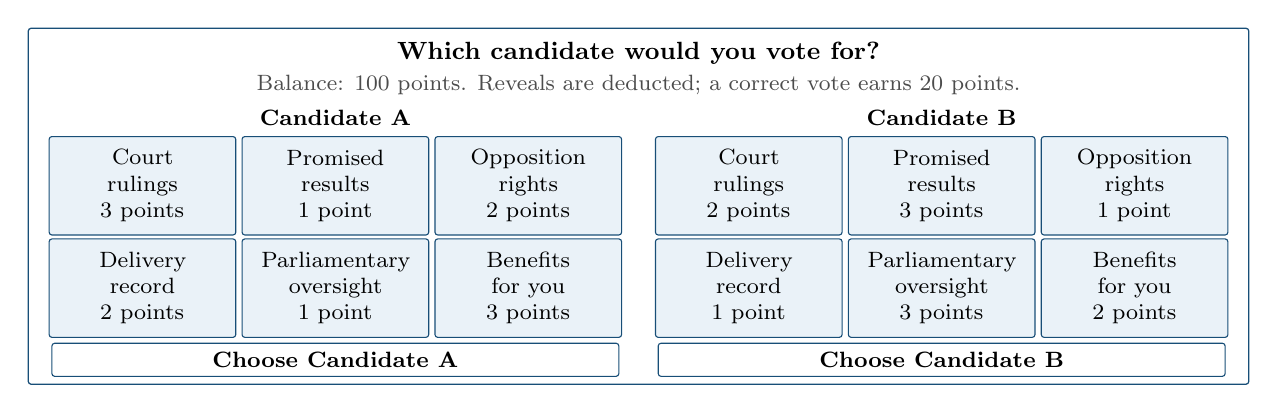
\begin{tikzpicture}[
  font=\footnotesize,
  tile/.style={draw=ecblue,fill=eclight,rounded corners=1pt,text width=2.3cm,minimum height=1.25cm,align=center,inner sep=1pt},
  choose/.style={draw=ecblue,rounded corners=1pt,minimum width=7.2cm,minimum height=0.42cm,align=center,inner sep=1.5pt,font=\footnotesize\bfseries}]
  \draw[draw=ecblue,rounded corners=1pt,line width=0.45pt] (-7.75,0.32) rectangle (7.75,-4.2);
  \node[font=\small\bfseries] at (0,0) {Which candidate would you vote for?};
  \node[text=black!70] at (0,-0.4) {Balance: 100 points. Reveals are deducted; a correct vote earns 20 points.};
  \node[font=\footnotesize\bfseries] at (-3.85,-0.82) {Candidate A};
  \node[font=\footnotesize\bfseries] at (3.85,-0.82) {Candidate B};
  \node[tile] at (-6.3,-1.68) {Court\\rulings\\3 points};
  \node[tile] at (-3.85,-1.68) {Promised\\results\\1 point};
  \node[tile] at (-1.4,-1.68) {Opposition\\rights\\2 points};
  \node[tile] at (-6.3,-2.98) {Delivery\\record\\2 points};
  \node[tile] at (-3.85,-2.98) {Parliamentary\\oversight\\1 point};
  \node[tile] at (-1.4,-2.98) {Benefits\\for you\\3 points};
  \node[choose] at (-3.85,-3.89) {Choose Candidate A};
  \node[tile] at (1.4,-1.68) {Court\\rulings\\2 points};
  \node[tile] at (3.85,-1.68) {Promised\\results\\3 points};
  \node[tile] at (6.3,-1.68) {Opposition\\rights\\1 point};
  \node[tile] at (1.4,-2.98) {Delivery\\record\\1 point};
  \node[tile] at (3.85,-2.98) {Parliamentary\\oversight\\3 points};
  \node[tile] at (6.3,-2.98) {Benefits\\for you\\2 points};
  \node[choose] at (3.85,-3.89) {Choose Candidate B};
\end{tikzpicture}
\caption{The economic conjoint choice screen. All six attributes of each candidate are hidden. Clicking a tile reveals the attribute and deducts its price. Three attributes concern democratic conduct and three concern results; tile positions and prices (1--3 points) are randomised in every choice.}
\label{fig:task}
\end{figure}

\begin{table}[!htbp]
\centering
\caption{Hidden attributes and planned levels}
\label{tab:attributes}
\footnotesize
\begin{tabularx}{\textwidth}{p{2.0cm} p{2.6cm} X X}
\toprule
\textbf{Class} & \textbf{Attribute} & \textbf{Level 1} & \textbf{Level 2} \\
\midrule
Democratic conduct ($\Dem$) & Court rulings & Will comply with court rulings that block government plans & Will set aside court rulings that block urgent action \\
 & Opposition rights & Will protect the opposition's right to delay and contest bills & Will limit opposition delays on urgent bills \\
 & Parliamentary oversight & Will submit major decisions to parliamentary scrutiny & Will act by decree when parliament delays \\
\midrule
Results ($\Res$) & Promised results & Promises to substantially reduce the problem within two years & Promises gradual improvement \\
 & Delivery record & Delivered most past promises & Delivered few past promises \\
 & Benefits for you & Your household would benefit from the candidate's programme & Your household would not be affected \\
\bottomrule
\end{tabularx}
\caption*{\footnotesize\textit{Notes:} Levels are illustrative and will be pretested in Finnish, Swedish and Spanish. ``The problem'' refers to the locally pretested urgent problem (organised crime in Chile, eastern-border security in Finland). Levels are assigned independently to each candidate.}
\end{table}

The incentive must make search consequential without telling respondents what to look for. A vote-choice question cannot do this: a stated preference cannot be right or wrong, so it cannot be rewarded, and a respondent who will not be rewarded has no reason to economise on information. Following \textcite{LauRedlawsk1997}, I therefore define a \emph{correct vote} as the choice the respondent would make with full information, given their own values. In Wave~1, respondents state, for each attribute, which level they prefer and how important the attribute is, by allocating 100 importance points across the six attributes. Let $w_{im}\geq 0$ denote respondent $i$'s importance weight for attribute $m$, with $\sum_m w_{im}=100$, and let $a_{ijtm}\in\{0,1\}$ indicate that candidate $j$ in choice $t$ carries the level that $i$ prefers on attribute $m$. Candidate $j$'s full-information value for $i$ is
\[
V_{ijt}=\sum_{m=1}^{6} w_{im}\,a_{ijtm},
\]
and the correct candidate is the one with the higher $V_{ijt}$. Candidate pairs are drawn so that $V_{iAt}\neq V_{iBt}$, which removes ties. Because weights are measured before treatment, the pairs are drawn identically in both arms.

The payoff structure follows \textcite{Downs1957}'s logic of costly political information. Each respondent starts with 100 points. A correct vote earns 20 points, an incorrect vote earns nothing, and each reveal costs between 1 and 3 points. Points convert to cash at a fixed rate at the end of the survey. Revealing all twelve tiles would cost 24 points on average, more than the reward. Voting blind therefore risks losing the reward, but revealing everything is never worthwhile. Respondents want to vote correctly, so they must buy information, and because they cannot profitably buy all of it, their purchases reveal what they consider decision-relevant. The rule is explained in neutral terms (``the correct candidate is the one that best matches the priorities you reported last week''), without restating those priorities, so that the task does not prime them. Feedback on correctness is withheld until the end, so that later choices are not shaped by learning from earlier outcomes. Payoff rules and price distributions are identical across arms, so incentives cannot produce a treatment effect.

\subsection{Randomisation}

Five features are randomised. First, the scenario $C_i\in\{0,1\}$ is assigned at the respondent level and held fixed across all ten choices. Second, attribute levels are drawn independently for each candidate and choice, subject to the no-tie constraint. Third, the price of each tile is drawn independently and uniformly from $\{1,2,3\}$ for every attribute, candidate and choice. Fourth, the screen positions of the six tiles are shuffled in every choice, so that position cannot be confounded with attribute class. Fifth, the side of the screen on which each candidate appears is random. The experiment is programmed in oTree, and every reveal is logged with its timestamp, price, position and order within the choice, together with the final vote, its correctness and the respondent's running balance.\footnote{An oTree prototype of the costly-reveal interface is available at \href{https://econ-conjoint-project.onrender.com/}{\texttt{econ-conjoint-project.onrender.com}}.}

%=====================================================================
\section{Quantities of interest}\label{sec:qoi}
%=====================================================================

\subsection{Notation}

Respondents are indexed by $i=1,\dots,N$, choices by $t=1,\dots,T$ with $T=10$, candidates by $j\in\{A,B\}$, and hidden attributes by $m\in\mathcal{M}=\Dem\cup\Res$, where $\Dem$ contains the three democratic-conduct attributes and $\Res$ the three results attributes. Let
\[
U_{ijtm}=
\begin{cases}
1 & \text{if respondent } i \text{ reveals attribute } m \text{ of candidate } j \text{ in choice } t,\\
0 & \text{otherwise,}
\end{cases}
\]
and let $P_{ijtm}\in\{1,2,3\}$ denote the randomised price of that tile. The dependent variable is not the value of the attribute but the decision to acquire it. Each respondent makes $2\times6\times10=120$ such decisions.

\subsection{Marginal information demand}

The design's core estimand is \emph{marginal information demand} (MID). In its general form, MID is the probability that attribute $m$ is revealed under a condition $z$ of substantive interest and a task condition $s$:
\[
\MID_m(z,s)=\Pr\bigl(U_{ijtm}=1 \mid Z=z,\; S=s\bigr).
\]
The conditioning variables can be defined at the respondent, choice or profile level, and need only be randomised or observed before acquisition. In the present application, the substantive condition is the scenario, $Z=C_i$, and the task condition is the tile's price, $S=P_{ijtm}$:
\[
\MID_m(c,p)=\Pr\bigl(U_{ijtm}=1 \mid C_i=c,\; P_{ijtm}=p\bigr).
\]
Averaging over the uniform price distribution gives the price-marginal quantity $\MID_m(c)=\tfrac{1}{3}\sum_{p=1}^{3}\MID_m(c,p)$, and averaging over attributes within a class gives class-level demand, $\MID_{\Dem}(c)=\tfrac{1}{3}\sum_{m\in\Dem}\MID_m(c)$ and $\MID_{\Res}(c)=\tfrac{1}{3}\sum_{m\in\Res}\MID_m(c)$. Because $C_i$ and $P_{ijtm}$ are randomised independently of each other and of all respondent characteristics, contrasts of MID across their values are causal.

\subsection{Effects of institutional crisis on search}

The attribute-specific effect of the crisis is
\[
\tau_m=\MID_m(1)-\MID_m(0),
\]
the change in the probability that attribute $m$ is bought when the institutional crisis is present rather than absent.

For each respondent, define total reveals and the share of reveals concerning democratic conduct,
\[
R_i=\sum_{t}\sum_{j}\sum_{m\in\mathcal{M}}U_{ijtm},
\qquad
S_i=\frac{\sum_{t}\sum_{j}\sum_{m\in\Dem}U_{ijtm}}{R_i},
\]
with potential outcomes $R_i(c)$ and $S_i(c)$. The primary estimand is the average treatment effect of the institutional crisis on the share of democratic reveals,
\[
\Delta_S=\E\bigl[S_i(1)-S_i(0)\bigr],
\]
reported together with the effect on total reveals,
\[
\Delta_R=\E\bigl[R_i(1)-R_i(0)\bigr].
\]
The pair $(\Delta_S,\Delta_R)$ is what distinguishes reallocation from disengagement (\cref{tab:predictions}). If crisis scales all search down in proportion, $\Delta_R<0$ but $\Delta_S=0$. H1 predicts $\Delta_S<0$ whatever the sign of $\Delta_R$.

Two clarifications follow. First, the additive analogue at the tile level,
\[
\gamma=\bigl[\MID_{\Dem}(1)-\MID_{\Res}(1)\bigr]-\bigl[\MID_{\Dem}(0)-\MID_{\Res}(0)\bigr],
\]
mirrors the difference-in-differences logic of standard interaction estimands and is expressed in probability units, but it is not by itself a test of reallocation. Under proportional disengagement by a factor $\kappa$, $\gamma=(\kappa-1)[\MID_{\Dem}(0)-\MID_{\Res}(0)]$, which is non-zero whenever baseline demand differs across classes. The relevant tile-level test is the ratio contrast
\[
\rho=\log\frac{\MID_{\Dem}(1)}{\MID_{\Res}(1)}-\log\frac{\MID_{\Dem}(0)}{\MID_{\Res}(0)},
\]
which is zero under proportional disengagement and negative under displacement. Since the aggregate share of democratic reveals in arm $c$ equals $\MID_{\Dem}(c)/[\MID_{\Dem}(c)+\MID_{\Res}(c)]$, $\rho$ and the aggregate version of $\Delta_S$ always have the same sign. I report $\gamma$ for interpretability and $\rho$ as the tile-level test of H1.

Second, $S_i$ is undefined for respondents who reveal nothing in all ten choices. Such respondents should be rare, because blind voting forgoes the expected reward, but their frequency may depend on treatment. I therefore report the effect of crisis on $\Pr(R_i=0)$, the always-defined aggregate share and tile-level ratio $\rho$, and, if zero-reveal rates differ across arms, trimming bounds on $\Delta_S$ \parencite{Lee2009bounds}.

\subsection{A causal demand curve for democratic information}

Because prices are randomised tile by tile, $\MID_m(c,p)$ traced over $p\in\{1,2,3\}$ is a causal demand curve for attribute $m$ in arm $c$. Its average slope is
\[
\eta_m(c)=\frac{\MID_m(c,3)-\MID_m(c,1)}{2},
\]
the change in the probability of purchase per additional point of price. The corresponding arc elasticity at the midpoint is
\[
\varepsilon_m(c)=\frac{\MID_m(c,3)-\MID_m(c,1)}{\MID_m(c,3)+\MID_m(c,1)}\cdot\frac{3+1}{3-1}.
\]
H2 concerns how crisis changes the slope of democratic demand relative to results demand:
\[
\kappa=\bigl[\eta_{\Dem}(1)-\eta_{\Dem}(0)\bigr]-\bigl[\eta_{\Res}(1)-\eta_{\Res}(0)\bigr],
\]
with H2 predicting $\kappa<0$: under crisis, information about restraint becomes a luxury that is dropped first when it is expensive. Because prices are also drawn independently for the two candidates, the design identifies cross-price effects. The effect of the rival candidate's price for attribute $m$ on revealing $m$ for candidate $j$ shows whether respondents treat the same information about the two candidates as complements, needing both to compare, or as substitutes. A comparative voter should treat them as complements.

The demand curve has a substantive interpretation that fully revealed designs lack. A high level of demand at low prices that collapses at high prices indicates that citizens value democratic information but not much; demand that is flat in price indicates that it is treated as a necessity. The difference between these two patterns, and whether crisis moves citizens from one to the other, is a direct measure of how much citizens are willing to pay to monitor restraint.

\subsection{Search relative to stated priorities}

Because the correct vote is defined by each respondent's own Wave-1 priorities, the design also yields a benchmark for how respondents \emph{should} search. Given $w_i$, the price draws and the known distribution of attribute levels, the expected-payoff-maximising search policy can be computed by backward induction over the twelve tiles of a choice: at each step, reveal the tile whose expected improvement in the probability of a correct vote, multiplied by the 20-point reward, most exceeds its price, or stop and vote. Let $S_i^{*}$ denote the democratic share of reveals under this policy, and define the search gap
\[
G_i=S_i-S_i^{*}.
\]
Since $S_i^{*}$ depends only on pre-treatment weights and randomised features, $\E[S_i^{*}(1)]=\E[S_i^{*}(0)]$, and the average effect of crisis on $G_i$ equals $\Delta_S$. The benchmark nonetheless adds two things. In levels, it shows whether respondents under-search democratic conduct relative to what their own priorities warrant in both arms, or only under crisis. In absolute value, $\E[|G_i(1)|-|G_i(0)|]$ shows whether crisis pushes search further from what respondents said matters, which is the normatively relevant sense of displacement. A simpler benchmark, the share of importance points allocated to democratic conduct, $\omega_i^{\Dem}=\sum_{m\in\Dem}w_{im}/100$, is reported alongside.

\subsection{Accuracy and earnings}

Let $Y_{it}\in\{0,1\}$ indicate a correct vote in choice $t$, and let $\pi_{it}=20\,Y_{it}-\sum_j\sum_m P_{ijtm}U_{ijtm}$ denote net earnings. The effects $\tau_Y=\E[\bar Y_i(1)-\bar Y_i(0)]$ and $\tau_\pi=\E[\bar\pi_i(1)-\bar\pi_i(0)]$, where bars denote averages over the ten choices, show whether displacement is costly. If crisis reallocates search away from attributes that respondents themselves weight heavily, it should reduce the probability of voting for the candidate they would have chosen with full information.

\subsection{Relation to AMCEs, marginal means and framing designs}

It is useful to distinguish these quantities from those of the standard conjoint framework. In \textcite{Hainmueller2014}, the principal estimand is the AMCE: the effect of changing attribute $\ell$ from level $x_0$ to $x_1$ on the probability that a profile is chosen, averaged over the distribution of the remaining attributes. \textcite{Leeper2020a} show that, in fully randomised designs, the AMCE is the difference between two marginal means, $\mathit{AMCE}_\ell(x_1,x_0)=\mathit{MM}_\ell(x_1)-\mathit{MM}_\ell(x_0)$, where $\mathit{MM}_\ell(x)=\Pr(Y_{ijt}=1\mid X_{ijt\ell}=x)$. Both quantities are defined over \emph{fully revealed} profiles and concern the \emph{final choice} (\cref{tab:estimands}).

\begin{table}[!htbp]
\centering
\caption{Standard conjoint estimands and the economic conjoint acquisition estimand}
\label{tab:estimands}
\footnotesize
\begin{tabularx}{\textwidth}{p{2.6cm} p{4.6cm} X p{2.6cm}}
\toprule
\textbf{Estimand} & \textbf{Notation} & \textbf{What it measures} & \textbf{Stage} \\
\midrule
AMCE \parencite{Hainmueller2014} & $\mathit{MM}_\ell(x_1)-\mathit{MM}_\ell(x_0)$ & Effect of changing attribute $\ell$ from $x_0$ to $x_1$ on profile choice, averaging over the remaining revealed attributes & Choice, given full exposure \\
Marginal mean \parencite{Leeper2020a} & $\Pr(Y=1\mid X_\ell=x)$ & Probability that a revealed profile with level $x$ is chosen & Choice, given full exposure \\
MID & $\Pr(U_{ijtm}=1\mid Z=z,S=s)$ & Probability that attribute $m$ is bought under condition $z$ and task condition $s$ & Acquisition, before choice \\
\bottomrule
\end{tabularx}
\caption*{\footnotesize\textit{Notes:} $Y$ denotes profile choice, $X_\ell$ a fully revealed attribute and $U_{ijtm}$ the decision to reveal attribute $m$ of candidate $j$ for respondent $i$ in choice $t$. MID is the acquisition-stage analogue of the marginal mean.}
\end{table}

These estimands do not compete with AMCEs or marginal means; they operate at an earlier stage of the decision. AMCEs and marginal means ask: \emph{once an attribute is part of the profile, how does it shape support?} MID asks: \emph{is the attribute acquired at all, under what conditions, and at what price?} The distinction also shows the limits of applying standard estimands to the present design. One could estimate the effect of a revealed court-ruling level on the final vote, but only among choices in which respondents chose to reveal it. Because revealing is itself affected by treatment, by prices and by previously revealed information, such conditional effects are subject to selection and are descriptive rather than causal. Standard conjoint estimands describe how information matters \emph{after} it enters the choice set; MID describes how it gets there.

Nor is the design a framing experiment. A framing design assigns one of a few externally imposed presentations, $F_i\rightarrow Y_i$, and a standard conjoint assigns a fully revealed attribute vector, $X_{ijt}\rightarrow Y_{ijt}$. The economic conjoint has the structure
\[
(C_i,\,P_{ijt})\;\longrightarrow\;U_{ijtm}\;\longrightarrow\;Y_{it},
\]
in which the information that enters the final judgement is jointly produced by randomised conditions and the respondent's own costly decisions.

%=====================================================================
\section{Estimation and inference}
%=====================================================================

\subsection{Specifications}

The primary respondent-level estimand $\Delta_S$ is estimated by regressing $S_i$ on the crisis indicator, with covariates centred and interacted with treatment \parencite{Lin2013}:
\[
S_i=\alpha+\Delta_S\,C_i+\boldsymbol{\beta}'\tilde{\mathbf{x}}_i+\boldsymbol{\theta}'(C_i\tilde{\mathbf{x}}_i)+u_i,
\]
where $\tilde{\mathbf{x}}_i$ contains centred pre-treatment covariates, chief among them the stated democratic share $\omega_i^{\Dem}$, together with task order and demographic quotas. Standard errors are heteroskedasticity-robust (HC2). Because $S_i$ is bounded in $[0,1]$, a fractional logit \parencite{PapkeWooldridge1996} is reported as a robustness check, and $\Delta_R$ is estimated with the same specification and $R_i$ as the outcome.

The tile-level MID quantities are estimated with attribute-specific linear probability models:
\[
U_{ijtm}=\alpha_m+\tau_m C_i+\sum_{p=2}^{3}\lambda_{mp}\,\mathbbm{1}[P_{ijtm}=p]+\sum_{p=2}^{3}\phi_{mp}\,C_i\,\mathbbm{1}[P_{ijtm}=p]+\delta_m L_{ijtm}+f_m(t)+\varepsilon_{ijtm},
\]
where $L_{ijtm}$ indicates the tile's screen position and side and $f_m(t)$ contains choice fixed effects. With the price indicators centred at their means, $\tau_m$ estimates $\MID_m(1)-\MID_m(0)$, the $\lambda_{mp}$ trace the control-arm demand curve, and the $\phi_{mp}$ estimate how crisis changes it. Estimating separate models for each attribute preserves the substantive meaning of each acquisition decision, since a higher probability of revealing court rulings does not mean the same as a higher probability of revealing personal benefits. Pooled models with class indicators, $\mathbbm{1}[m\in\Dem]$, and their interactions with $C_i$ and price estimate $\gamma$ and $\kappa$; a Poisson pseudo-likelihood model on class-level counts estimates $\rho$ as the coefficient on the interaction between crisis and democratic class.

The main MID models condition only on randomised features and on pre-treatment covariates. They do not condition on the values of attributes revealed earlier in the same choice, on earlier choices' outcomes or on the running balance, all of which are post-treatment. The rival candidate's price for the same attribute enters only in the cross-price model. Sequential search patterns, such as whether respondents stop after a decisive democratic attribute, are analysed descriptively.

\subsection{Inference}

Because the same respondent makes 120 acquisition decisions, tile-level standard errors are clustered by respondent, the unit at which the crisis is assigned. Randomisation inference, permuting $C_i$ across respondents within country, provides design-based $p$-values for $\Delta_S$, $\Delta_R$ and $\rho$ \parencite{GerberGreen2012,ImbensRubin2015}. Holm corrections are applied within hypothesis families \parencite{Holm1979}: the six attribute-specific $\tau_m$, and the six slope contrasts underlying H2. Country estimates are primary. Pooled estimates require measurement invariance of the priority and manipulation-check items after translation, back-translation and cognitive interviewing. The moderators in H3, institutional trust and authoritarian predisposition, are measured in Wave~1 and analysed as preregistered interactions with $C_i$. Respondents who fail the attention checks embedded in Wave~1 are excluded before randomisation, so no exclusion is conditioned on treatment.

\subsection{Power}

With 750 respondents per arm in each country, a two-sided test at $\alpha=0.05$ has 80\% power to detect a standardised effect on $S_i$ of
\[
(z_{0.975}+z_{0.80})\sqrt{\tfrac{1}{750}+\tfrac{1}{750}}=2.80\times0.052\approx0.15\ \text{SD},
\]
and about 0.10~SD in the pooled sample. Covariate adjustment for $\omega_i^{\Dem}$, which should strongly predict $S_i$, will reduce these minimum detectable effects further. If the respondent-level share has a standard deviation of about 0.20, 0.15~SD corresponds to a shift of three percentage points in the share of search devoted to democratic conduct. The demand-curve quantities are estimated with greater precision because prices vary within respondent: each country yields $1{,}500\times120=180{,}000$ priced acquisition decisions, so the slope contrasts in H2 are identified from within-respondent variation that is unaffected by between-respondent heterogeneity in overall search.

\subsection{Preregistration, ethics and openness}

All confirmatory tests, exclusion rules, the optimal-search algorithm and the moderators will be preregistered before Wave~2 fieldwork, following a pilot that checks the scenarios' strength, the distribution of reveals and the rate of zero-reveal respondents. The study follows the Finnish National Board on Research Integrity (TENK) guidelines and Chilean requirements, with ethics review before piloting. Respondents give informed consent, may withdraw without penalty and are debriefed; the crisis scenarios are pretested for distress. Earnings depend only on correctness and reveals, never on which candidate is chosen. Code, materials in all three languages and anonymised data will be released in this paper's public repository.

%=====================================================================
\section{Results}
%=====================================================================

Data collection has not yet taken place, so this section describes what will be reported. The first figure will plot $\MID_m(c)$ for each of the six attributes by arm and country, with the attribute-specific effects $\tau_m$. The first table will report $\Delta_S$ and $\Delta_R$, with randomisation-inference $p$-values, the ratio contrast $\rho$, and the effect on zero-reveal rates, which together adjudicate between the accounts in \cref{tab:predictions}. A second figure will plot the demand curves $\MID_{\Dem}(c,p)$ and $\MID_{\Res}(c,p)$ for H2, and a second table will report search gaps relative to the payoff-maximising benchmark, accuracy and earnings, followed by the moderation tests for H3.

\clearpage
\singlespacing
\printbibliography

\end{document}
